\documentclass[accentcolor=tud8b,colorbacktitle]{tudbeamer}

\usepackage[utf8]{inputenc}
\usepackage{graphicx}
\usepackage{subfig}
\usepackage{multicol}
\usepackage[most]{tcolorbox}
\usepackage{wasysym}

\title{\textcolor{white}{Collide, Collate, Collect: Recognizing Senders in Wireless Collisions\\}}
\subtitle{\textcolor{white}{B.Sc. Thesis Final Presentation\\Johannes Lauinger}}
\author{SEEMOO | Bachelor Thesis Final Presentation | Johannes Lauinger}
\logo{
\includegraphics{../../gfx/logos/seemoo-logo}}
\date{16.08.2017}


\begin{document}

\begin{titleframe}
	%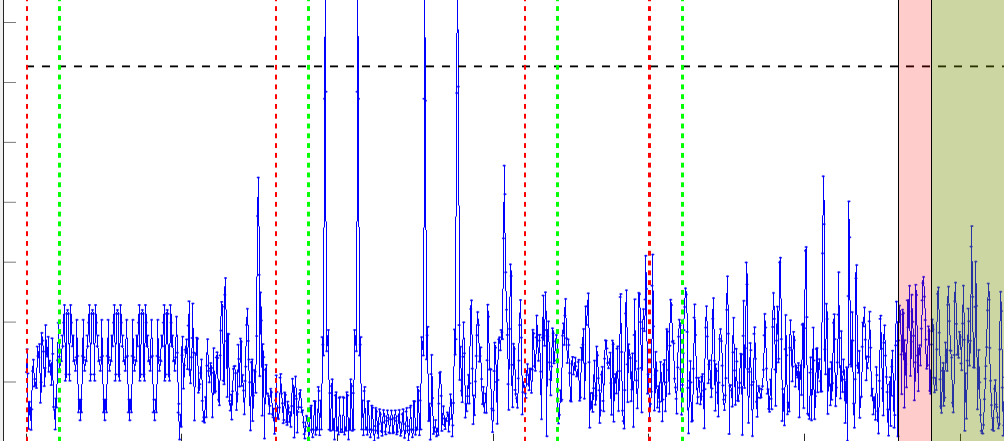
\includegraphics[width=12.1cm]{assets/title-image}
\end{titleframe}


\begin{frame}
\frametitle{Outline}
\begin{itemize}
	\setlength\itemsep{1em}
	\item Motivation
	\item Background
	\item Related Work
	\item Detector Design
	\item Evaluation Results
	\item Live Demo
	\item Discussion \& Conclusion
\end{itemize}
\end{frame}


\begin{frame}
\frametitle{Motivation}
\begin{itemize}
	\setlength\itemsep{1em}
	\item Collisions exist in IEEE 802.11 networks despite counter-measures
	\item Easy to spot a collision
	\item Hard to detect \textbf{which senders} collided \cite{choi2013, keene2010}
	\item Useful for improvements to the coordination function
	\item Example: A and B collide $\rightarrow$ C is next up for sending
	\item Also: statistics, network monitoring
\end{itemize}
\end{frame}


\begin{frame}
\frametitle{Background}
\begin{centering}
	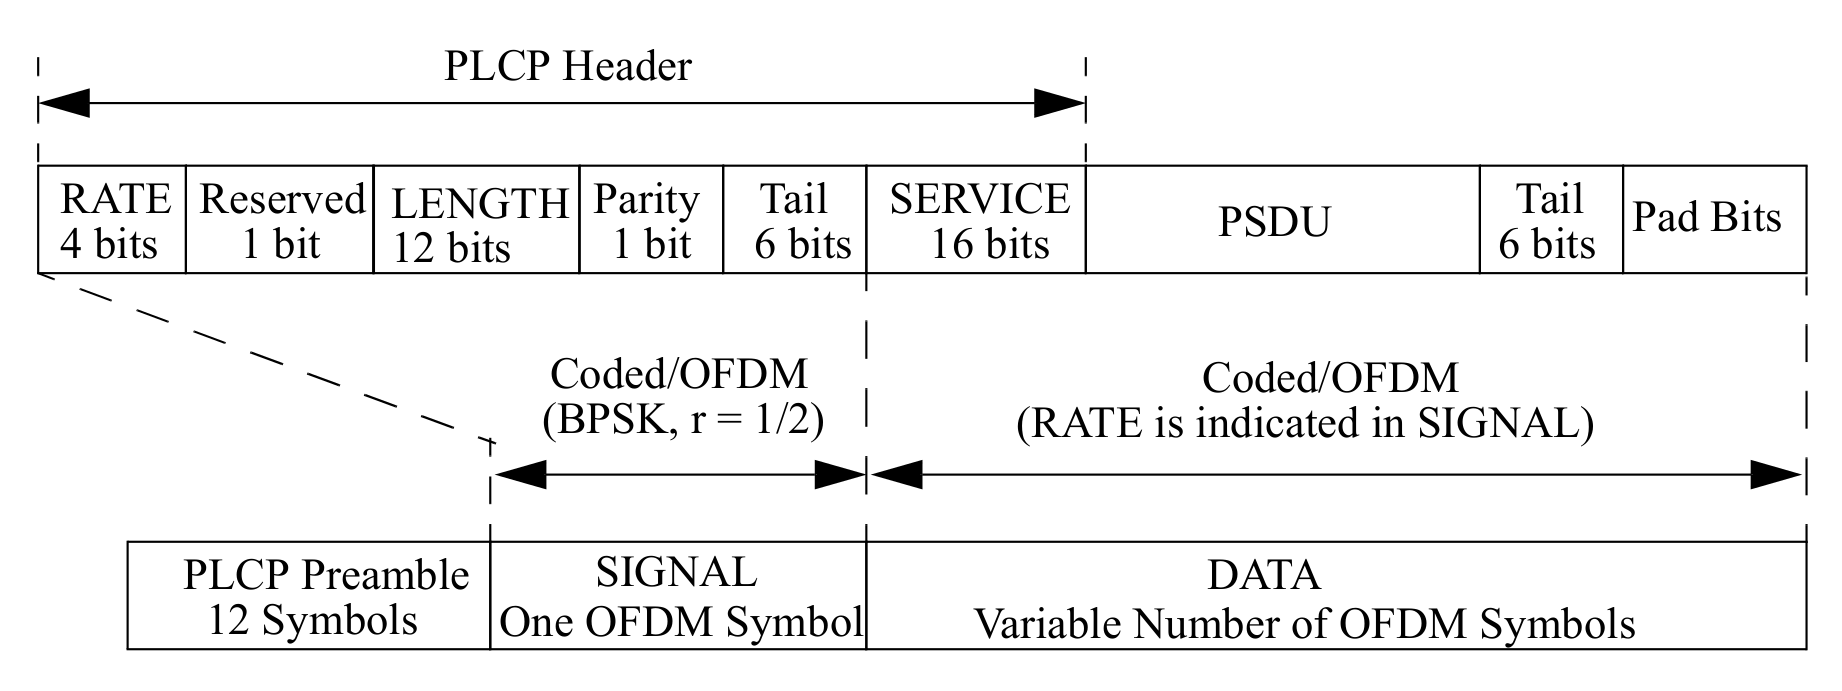
\includegraphics[width=8.5cm]{assets/phy-format}\\
	\vspace{0.3cm}
	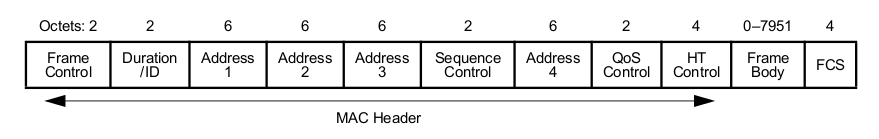
\includegraphics[width=\textwidth]{assets/mac-format}\\
	\small Figures: \cite{ieee2012} \normalsize\\~\\
\end{centering}
\end{frame}


\begin{frame}
\frametitle{Related Work}
\begin{itemize}
	\setlength\itemsep{1em}
	\item ZigZag \cite{gollakota2008} collision decoding
	\item Onion Decoding \cite{wang2010} for broadcast frames
	\item ReCoder \cite{meng2015} cross-correlation neighbor discovery
	\vspace{0.2cm}
	\item Problem: MAC Layer implementation change
\end{itemize}
\end{frame}


\begin{frame}
\frametitle{Detector Design}
\begin{centering}
	\vspace{0.7cm}
	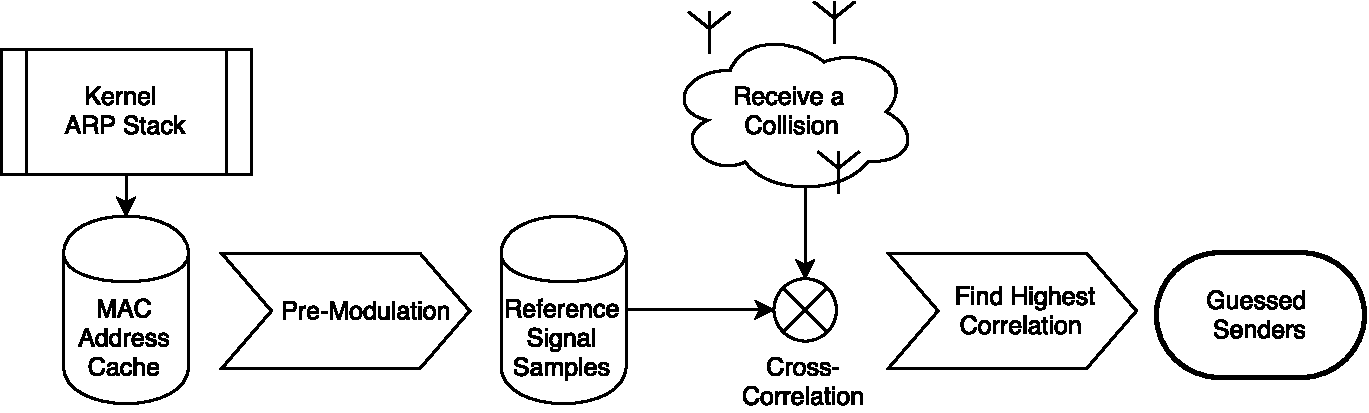
\includegraphics[width=\textwidth]{assets/detector-block-design}\\
\end{centering}
\end{frame}


\begin{frame}
\frametitle{Detect a Collision}
\begin{centering}
	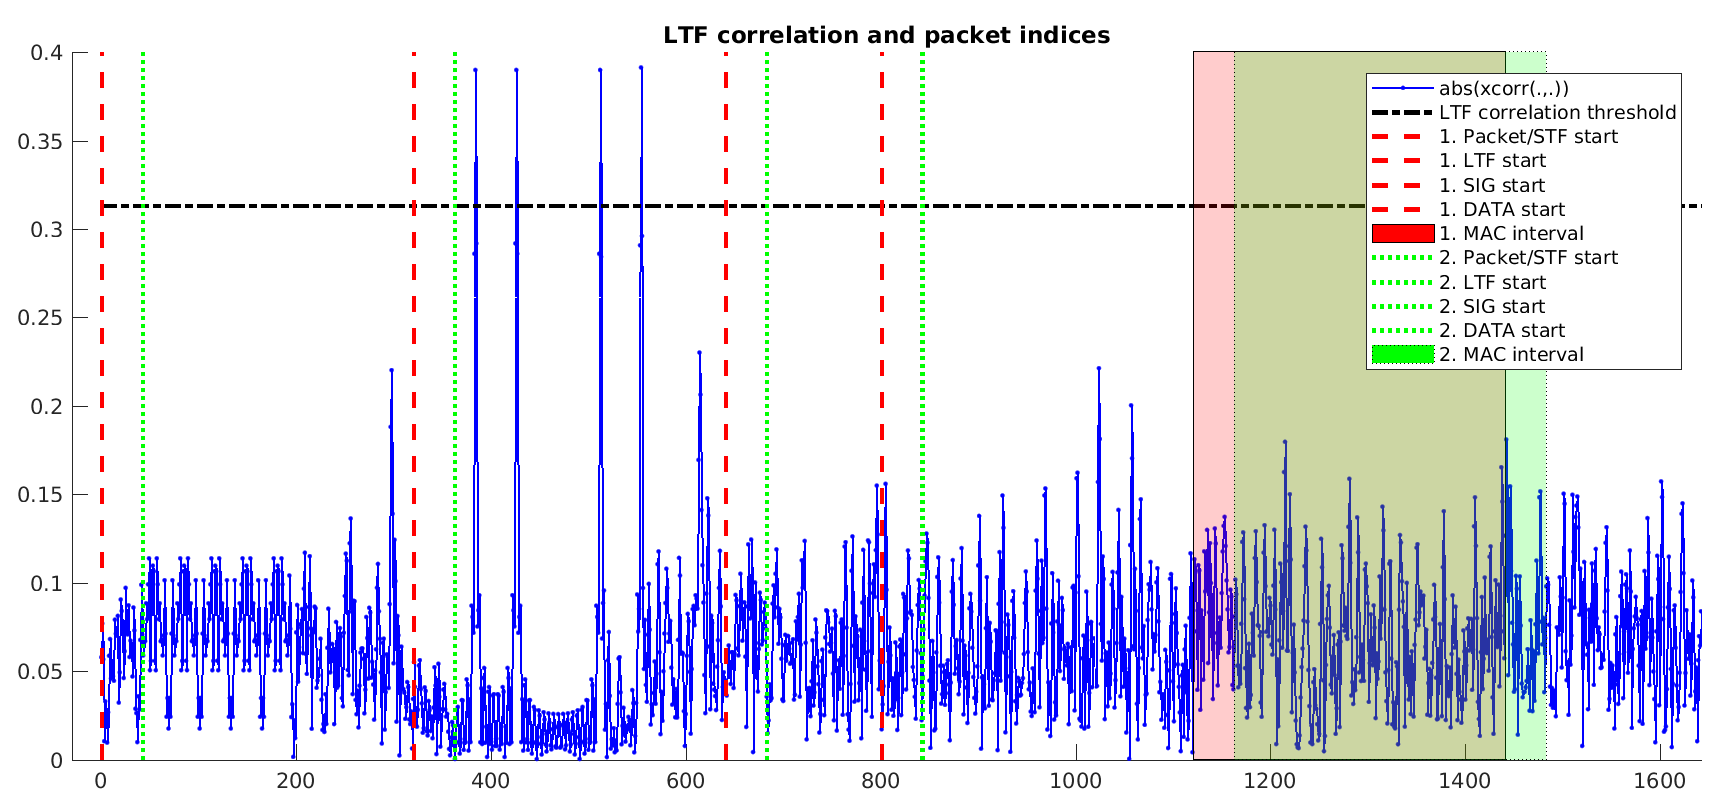
\includegraphics[width=\textwidth]{assets/preamble}\\
\end{centering}
\end{frame}


\begin{frame}
\frametitle{Evaluation}
\begin{itemize}
	\setlength\itemsep{1em}
	\item Simulation and WARP SDR experiments
	\item Implementation optimizations:
	\begin{itemize}
		\item Placeholder Frame Check Sequence (FCS) 0x42424242
		\item No preamble modulation
		\item Reference signal cache
	\end{itemize}
	\item Evaluation:
	\begin{itemize}
		\item Multiple experiment runs
		\item Different sender MAC addresses
		\item Count runs with \{0,1,2\} correct guesses
		\item Plot stacked sums
	\end{itemize}
\end{itemize}
\end{frame}


\begin{frame}
\frametitle{Results: Different MCSs}
\begin{centering}
	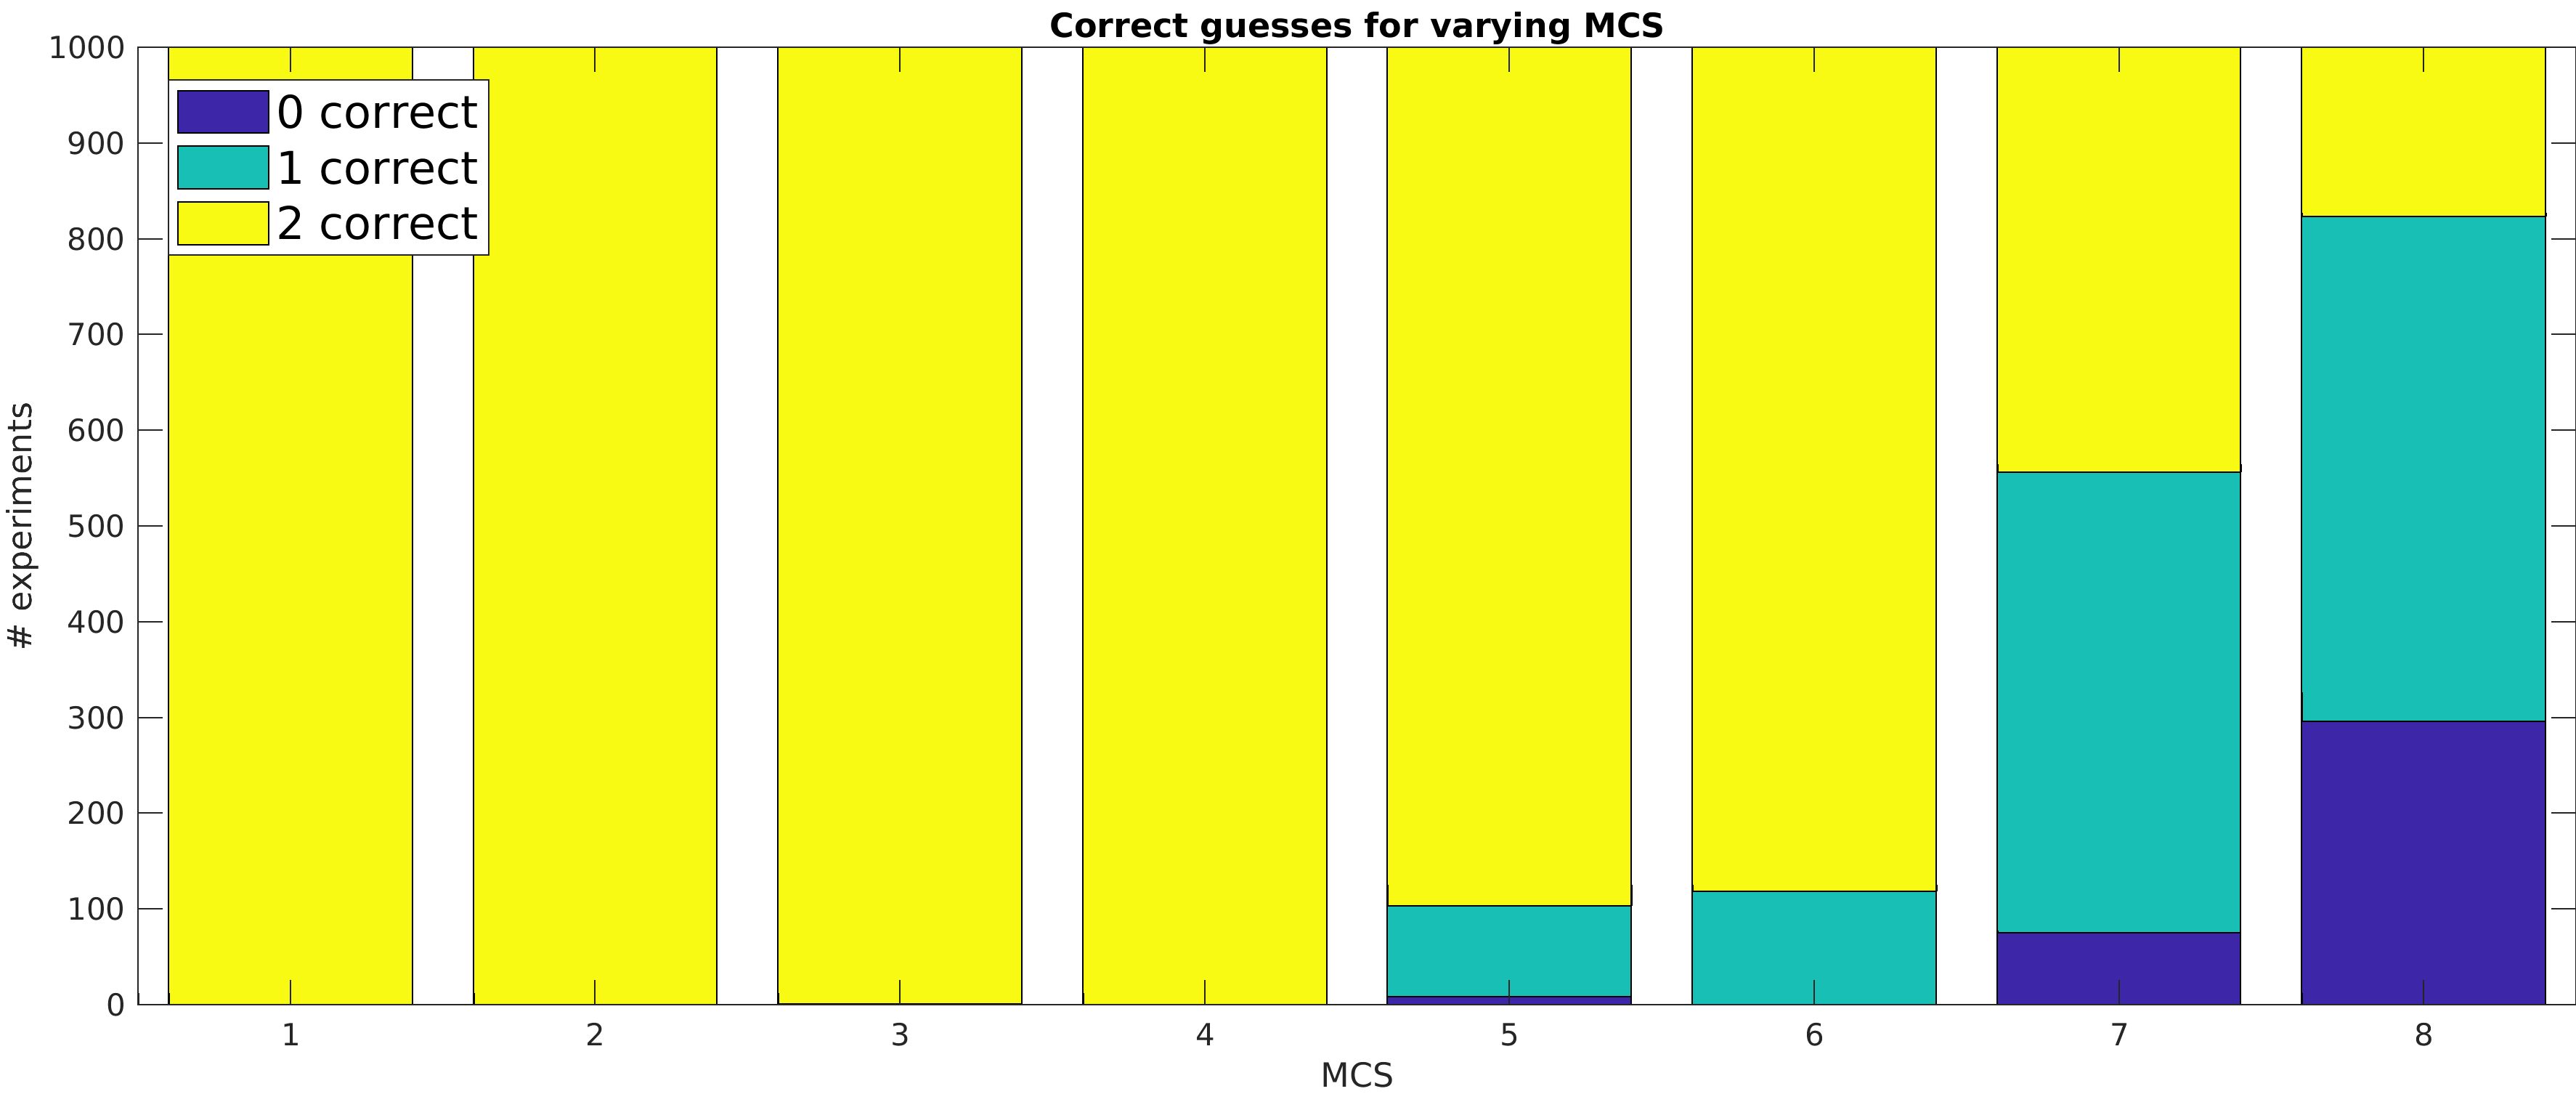
\includegraphics[width=\textwidth]{../../gfx/plots/mcs}\\
\end{centering}
\end{frame}


\begin{frame}
\frametitle{Results: Scrambler Initialization}
\begin{centering}
	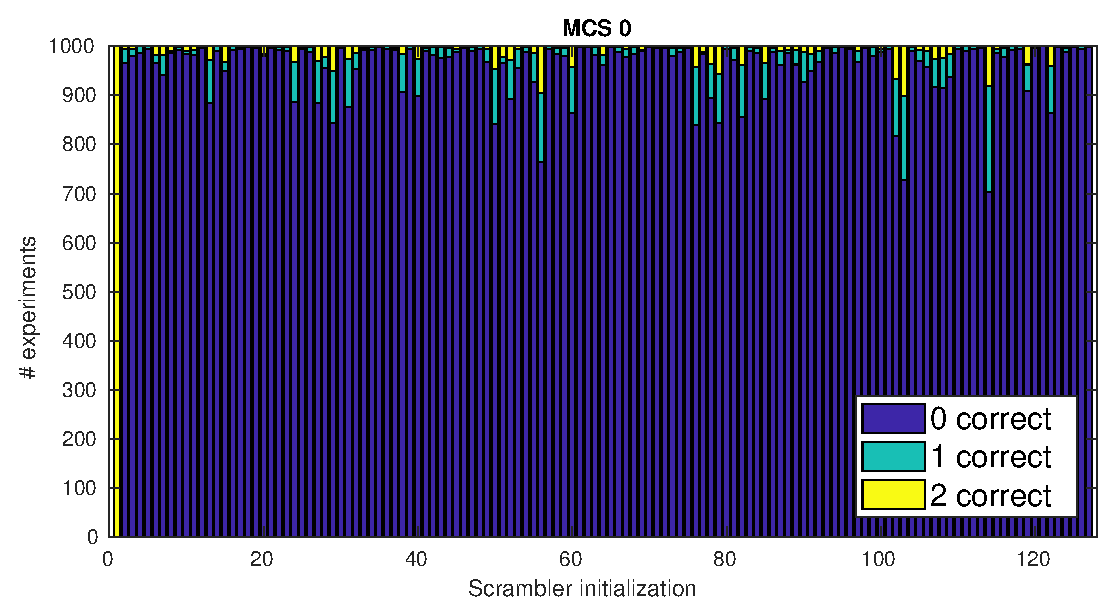
\includegraphics[width=11cm]{../../gfx/plots/scrambler}\\
\end{centering}
\end{frame}


\begin{frame}
\frametitle{Results: Destination MAC Address}
\begin{centering}
	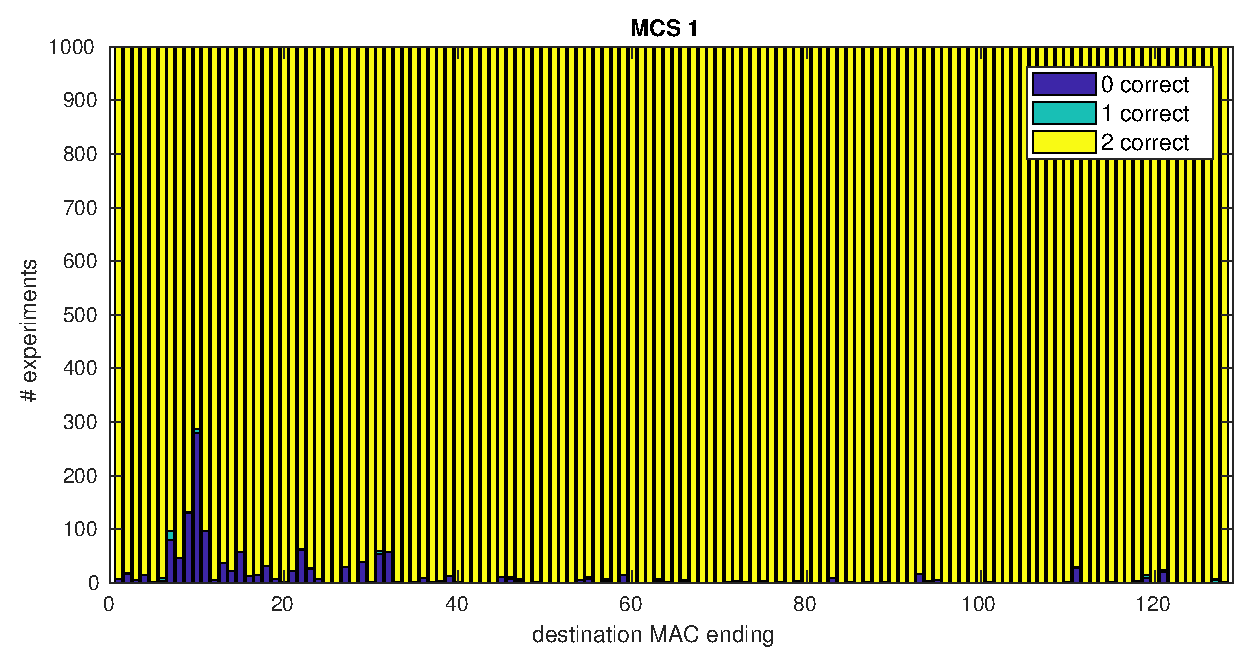
\includegraphics[width=11cm]{../../gfx/plots/destination}\\
\end{centering}
\end{frame}


\begin{frame}
\frametitle{Results: AWGN Channel}
	\centering
	\vspace{-0.3cm}
	\begin{tabular}{cc}
		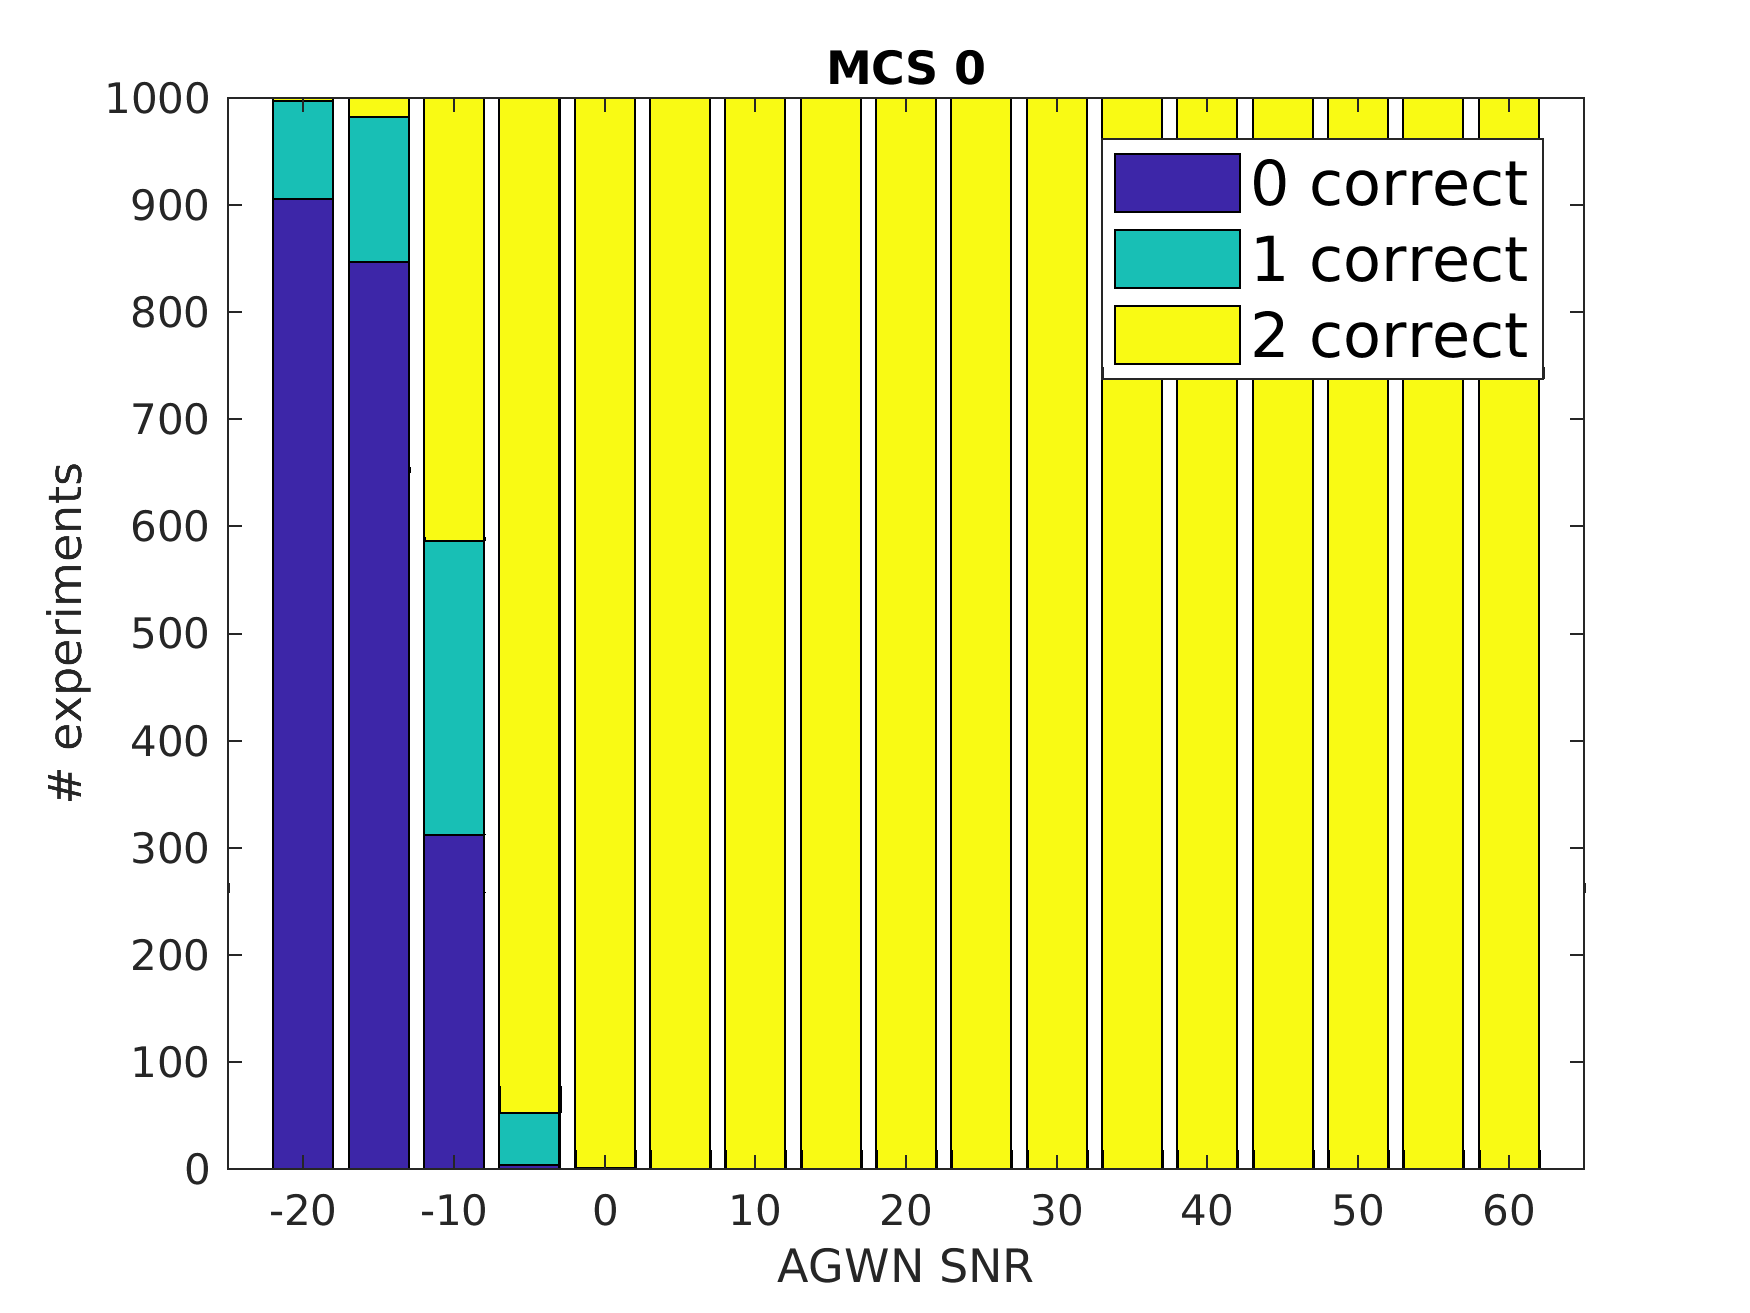
\includegraphics[height=0.52\textheight]{../../gfx/plots/awgn-mcs0} &
		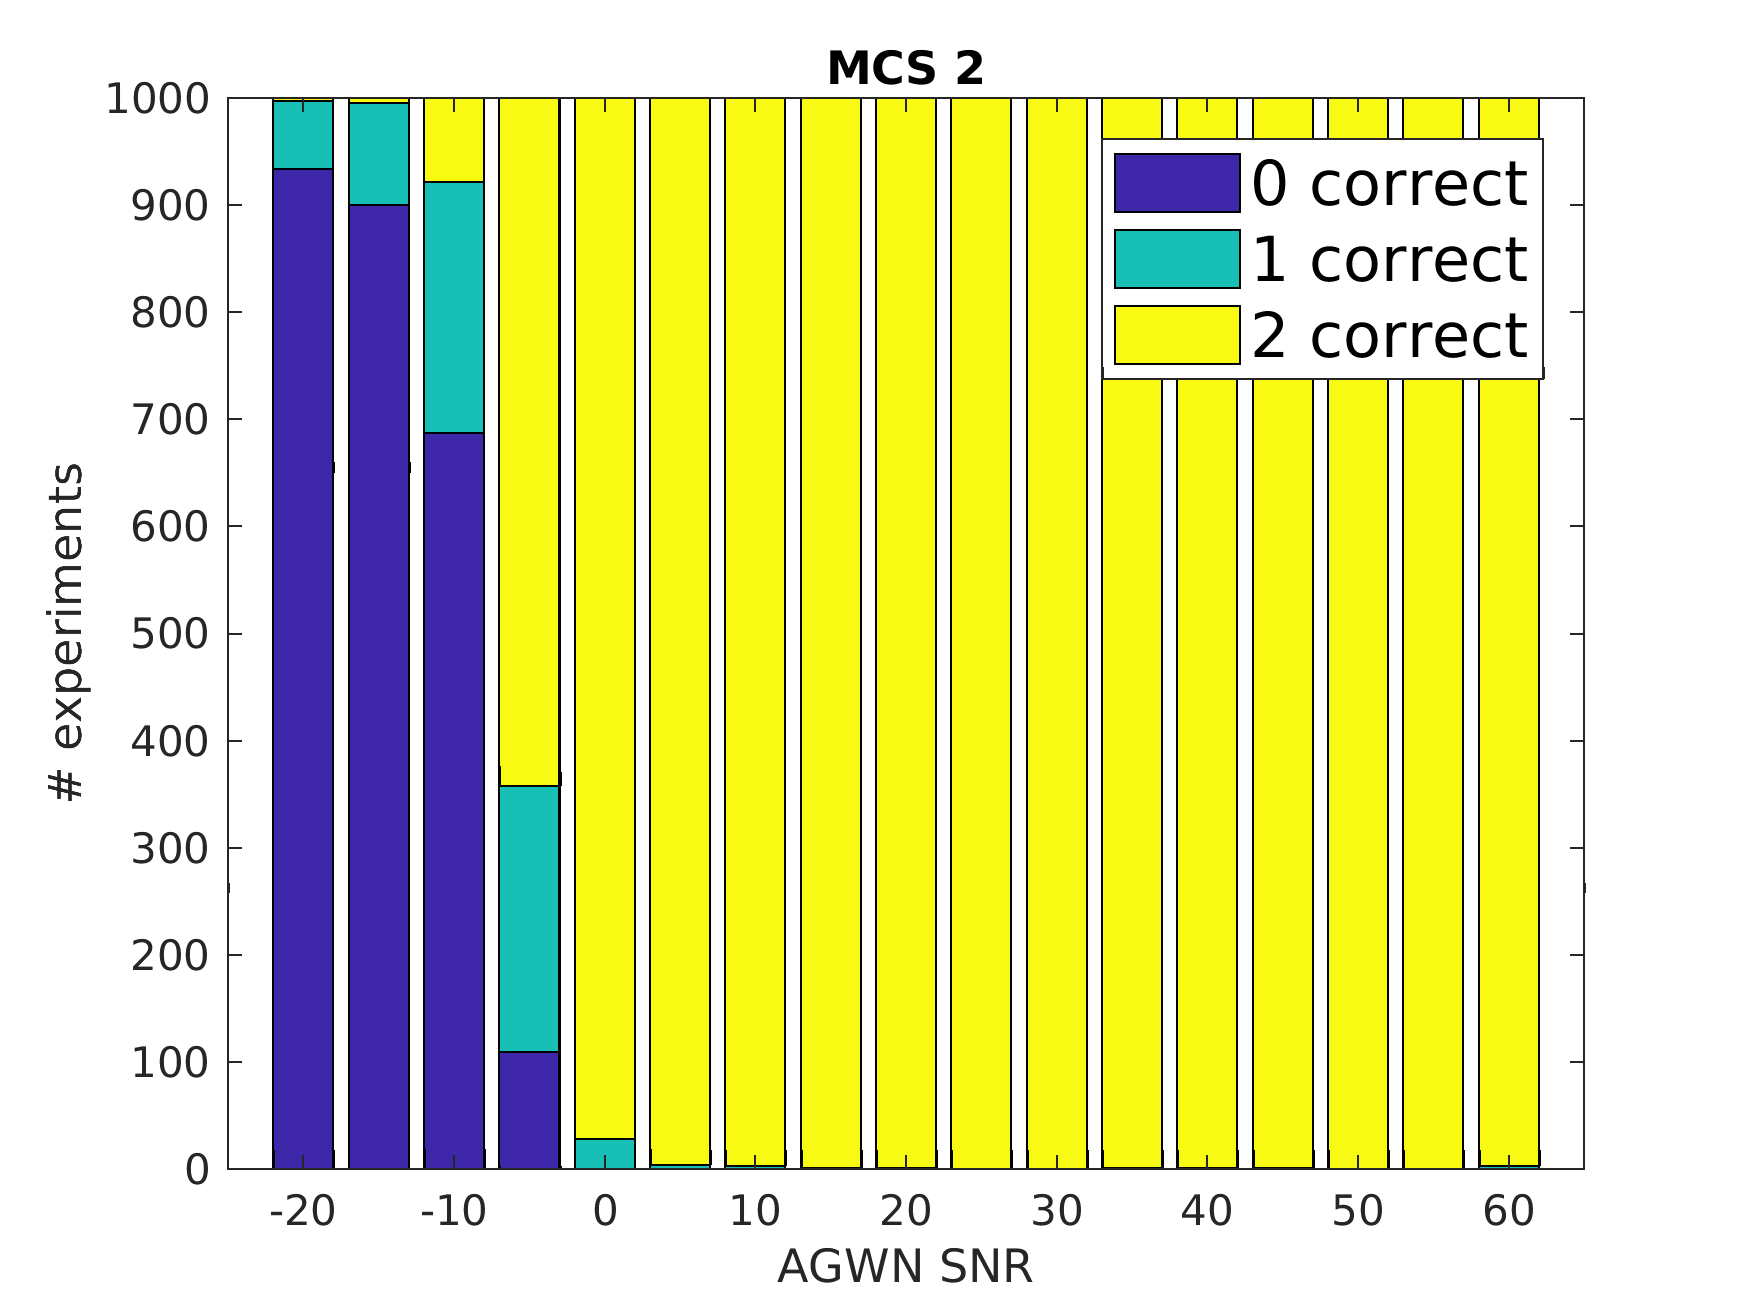
\includegraphics[height=0.52\textheight]{../../gfx/plots/awgn-mcs2} \\
		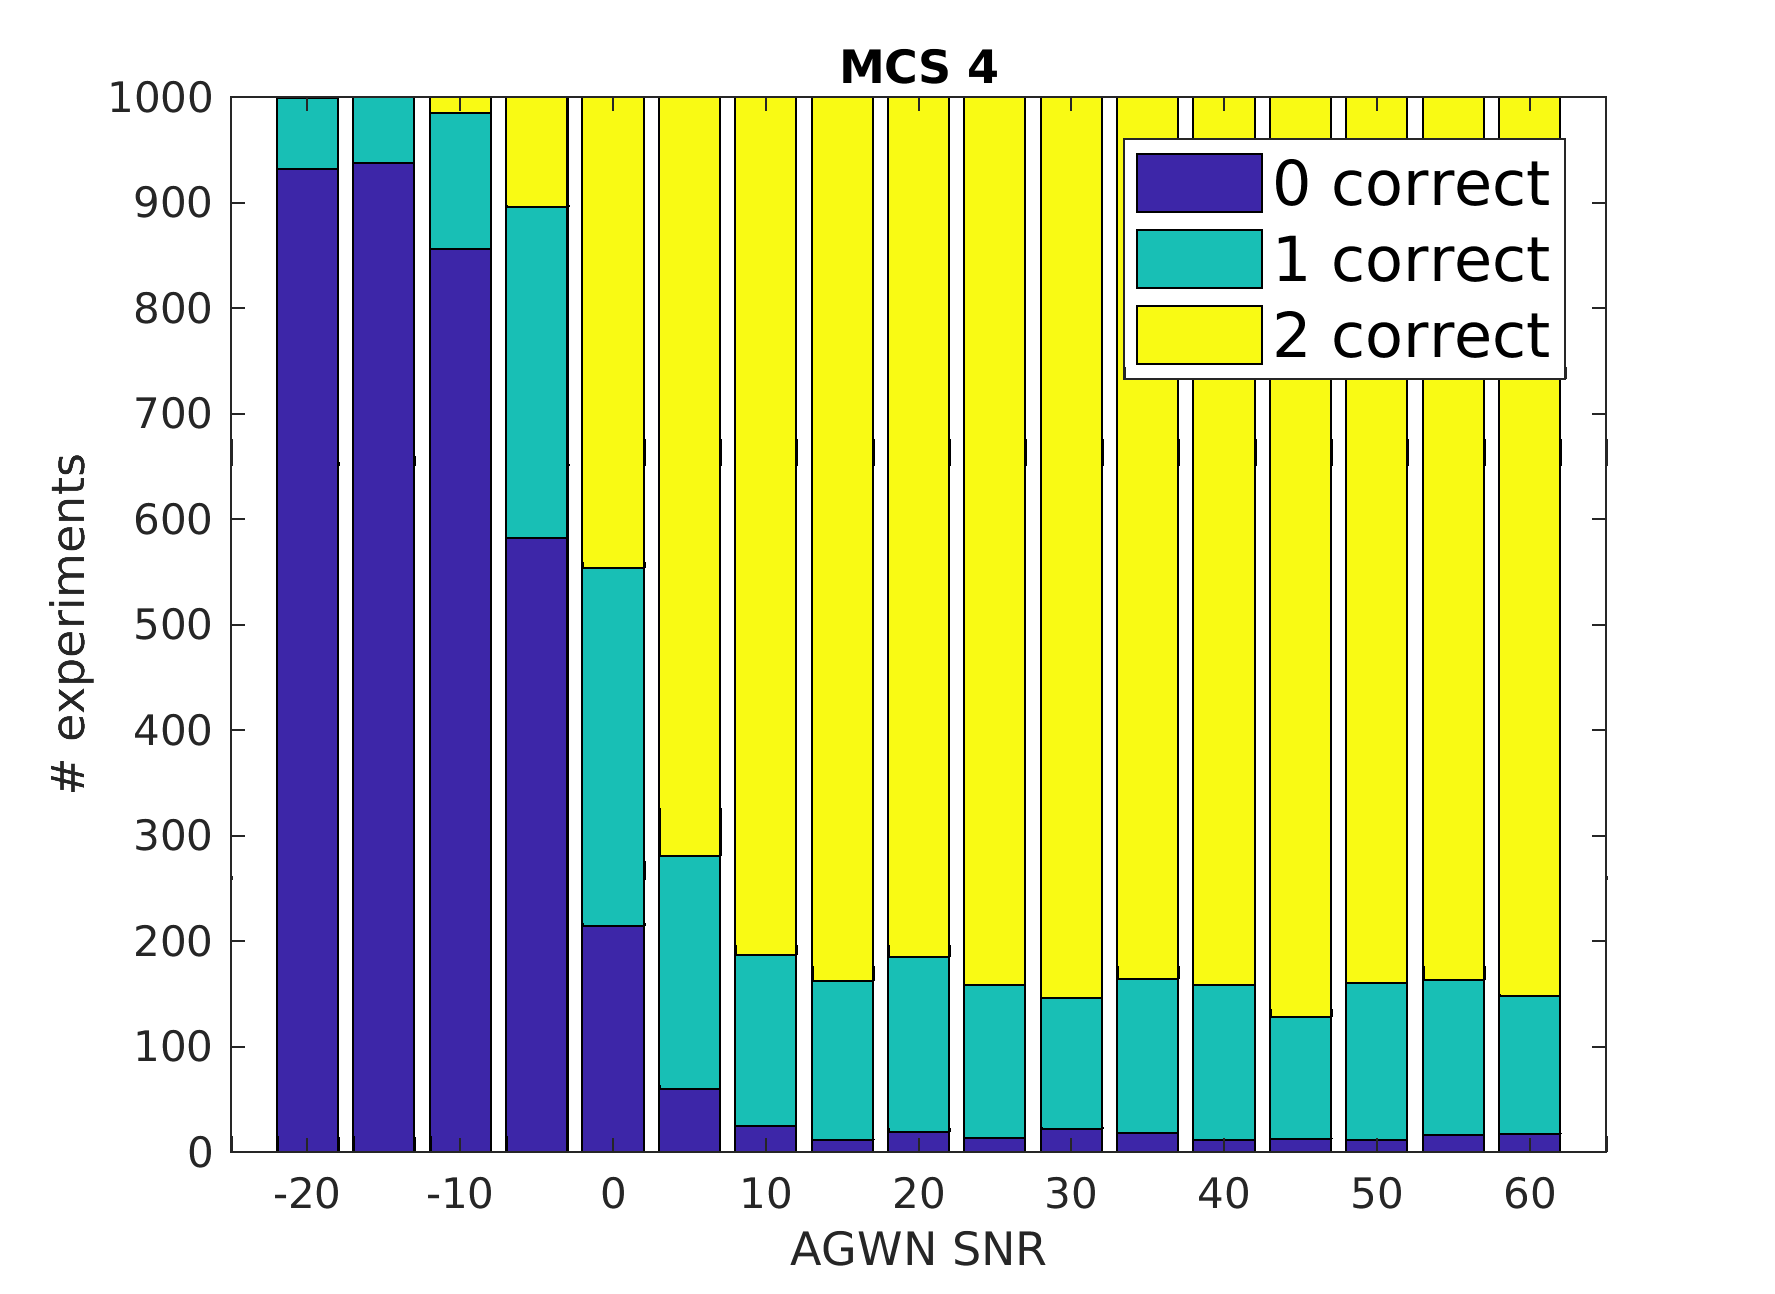
\includegraphics[height=0.52\textheight]{../../gfx/plots/awgn-mcs4} &
		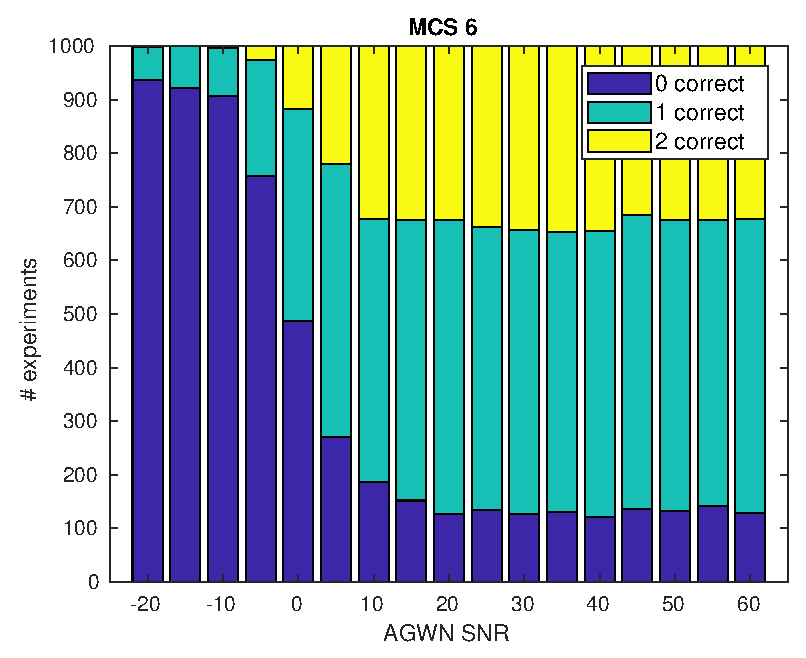
\includegraphics[height=0.52\textheight]{../../gfx/plots/awgn-mcs6} \\
	\end{tabular}
\end{frame}


\begin{frame}
\frametitle{Results: stdchan t$_\text{RMS}$}
\begin{figure}[H]
	\centering
	\vspace{-0.5cm}
	\begin{tabular}{cc}
		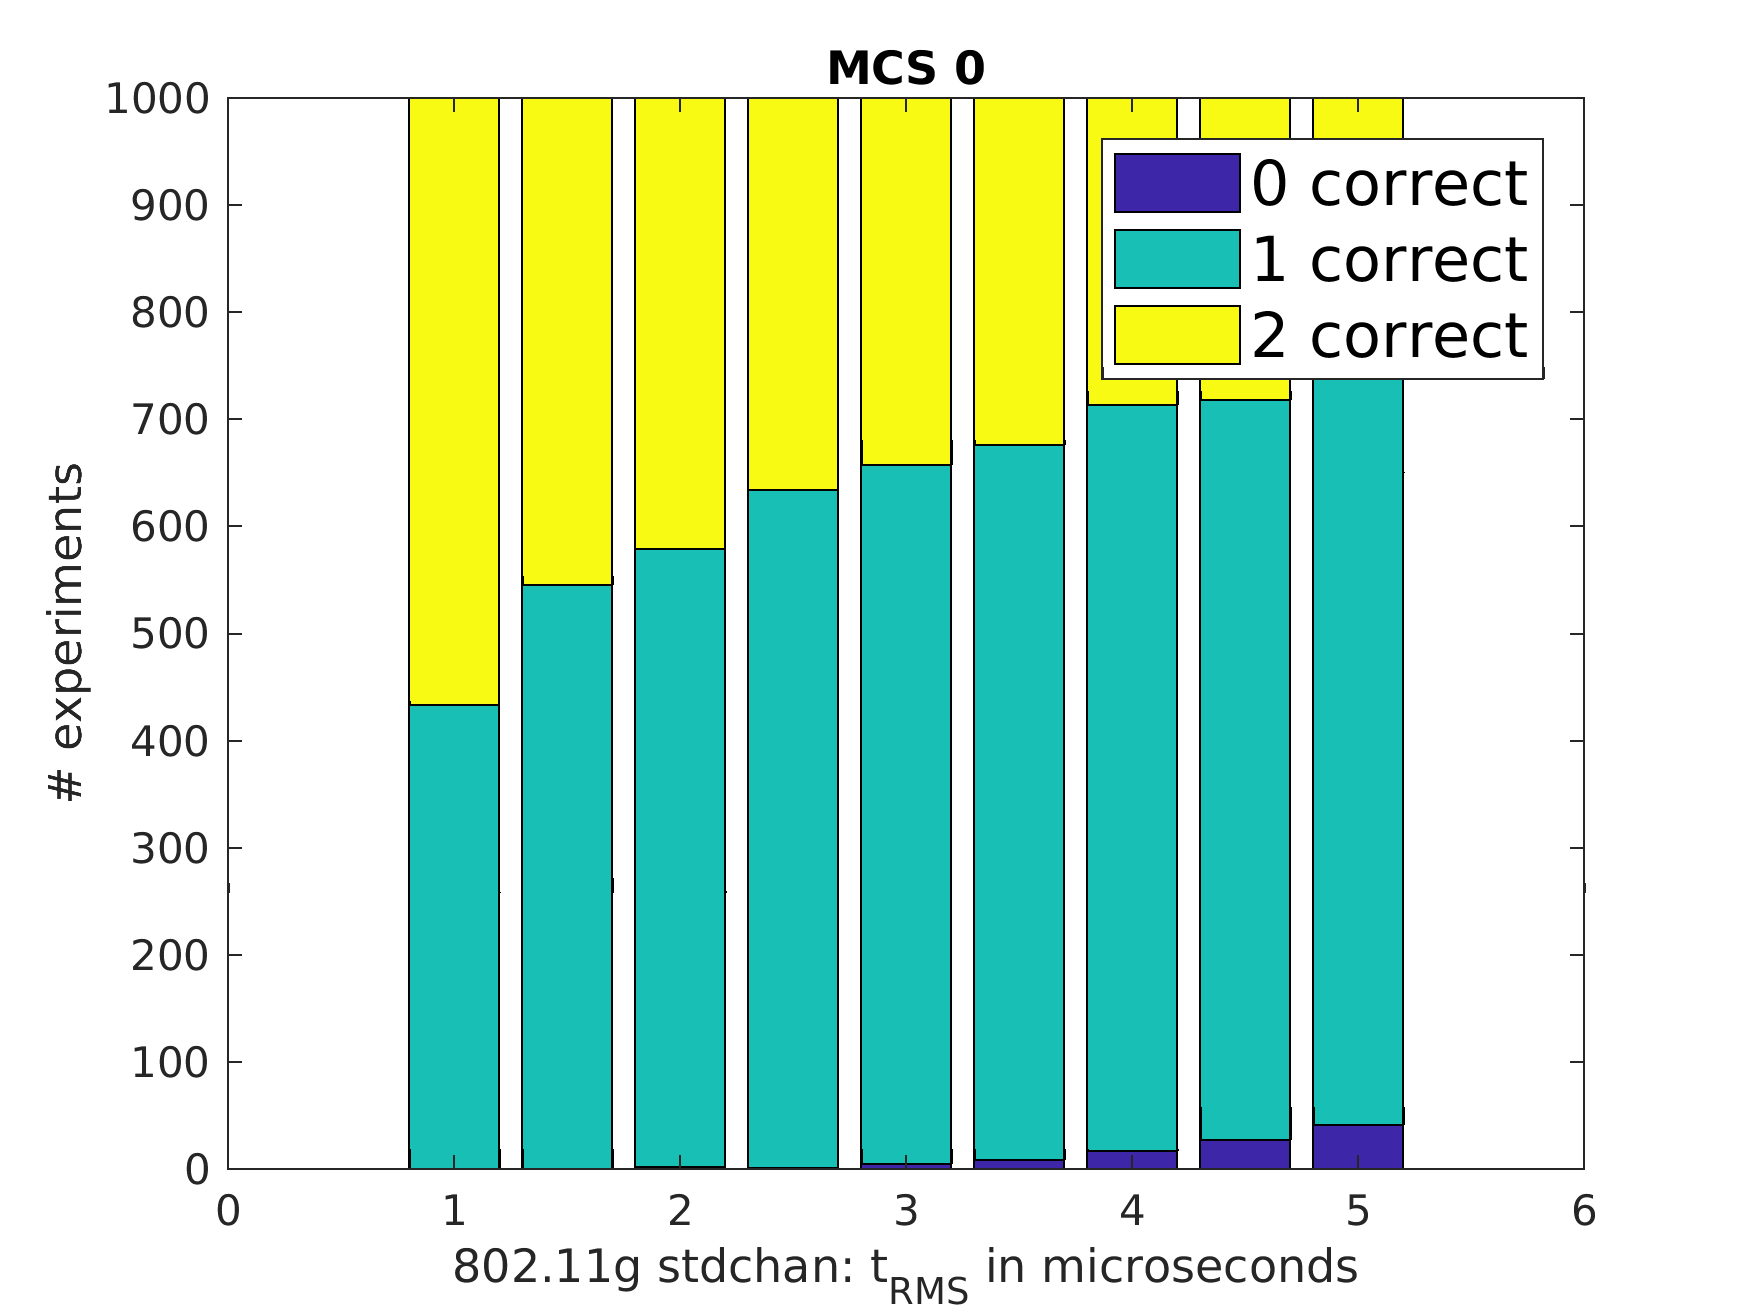
\includegraphics[height=0.52\textheight]{../../gfx/plots/trms-mcs0} &
		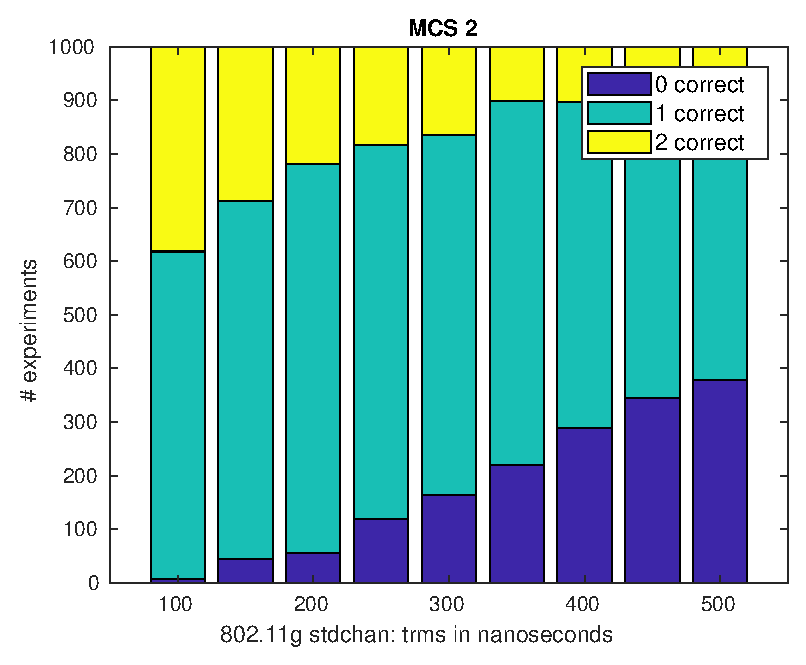
\includegraphics[height=0.52\textheight]{../../gfx/plots/trms-mcs2} \\
		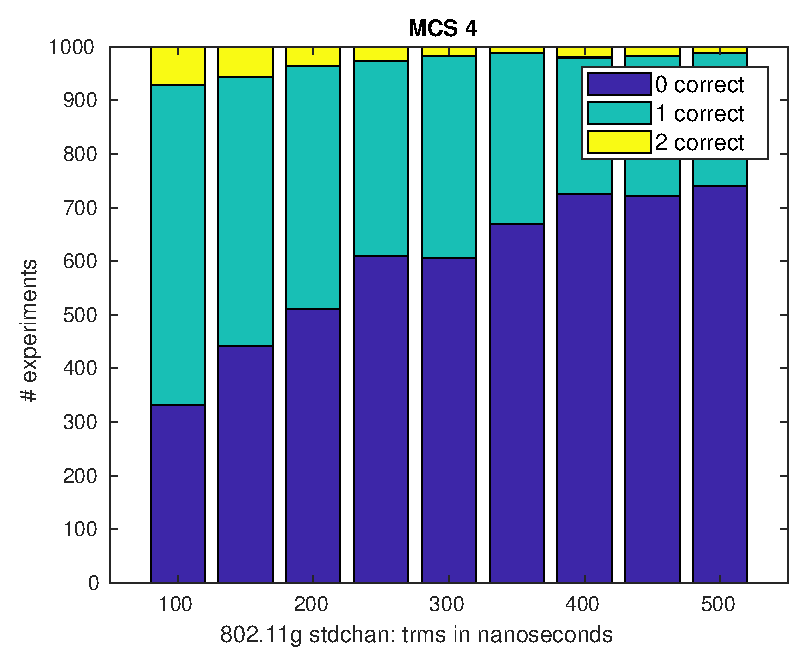
\includegraphics[height=0.52\textheight]{../../gfx/plots/trms-mcs4} &
		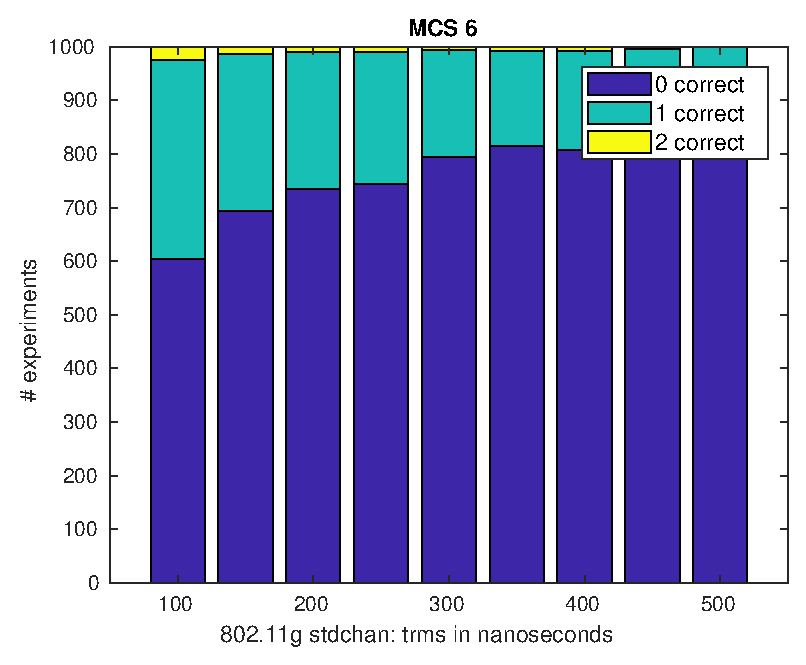
\includegraphics[height=0.52\textheight]{../../gfx/plots/trms-mcs6} \\
	\end{tabular}
\end{figure}
\end{frame}


\begin{frame}
\frametitle{Results: TGn Channel}
\begin{figure}[H]
	\centering
	\vspace{-0.5cm}
	\begin{tabular}{cc}
		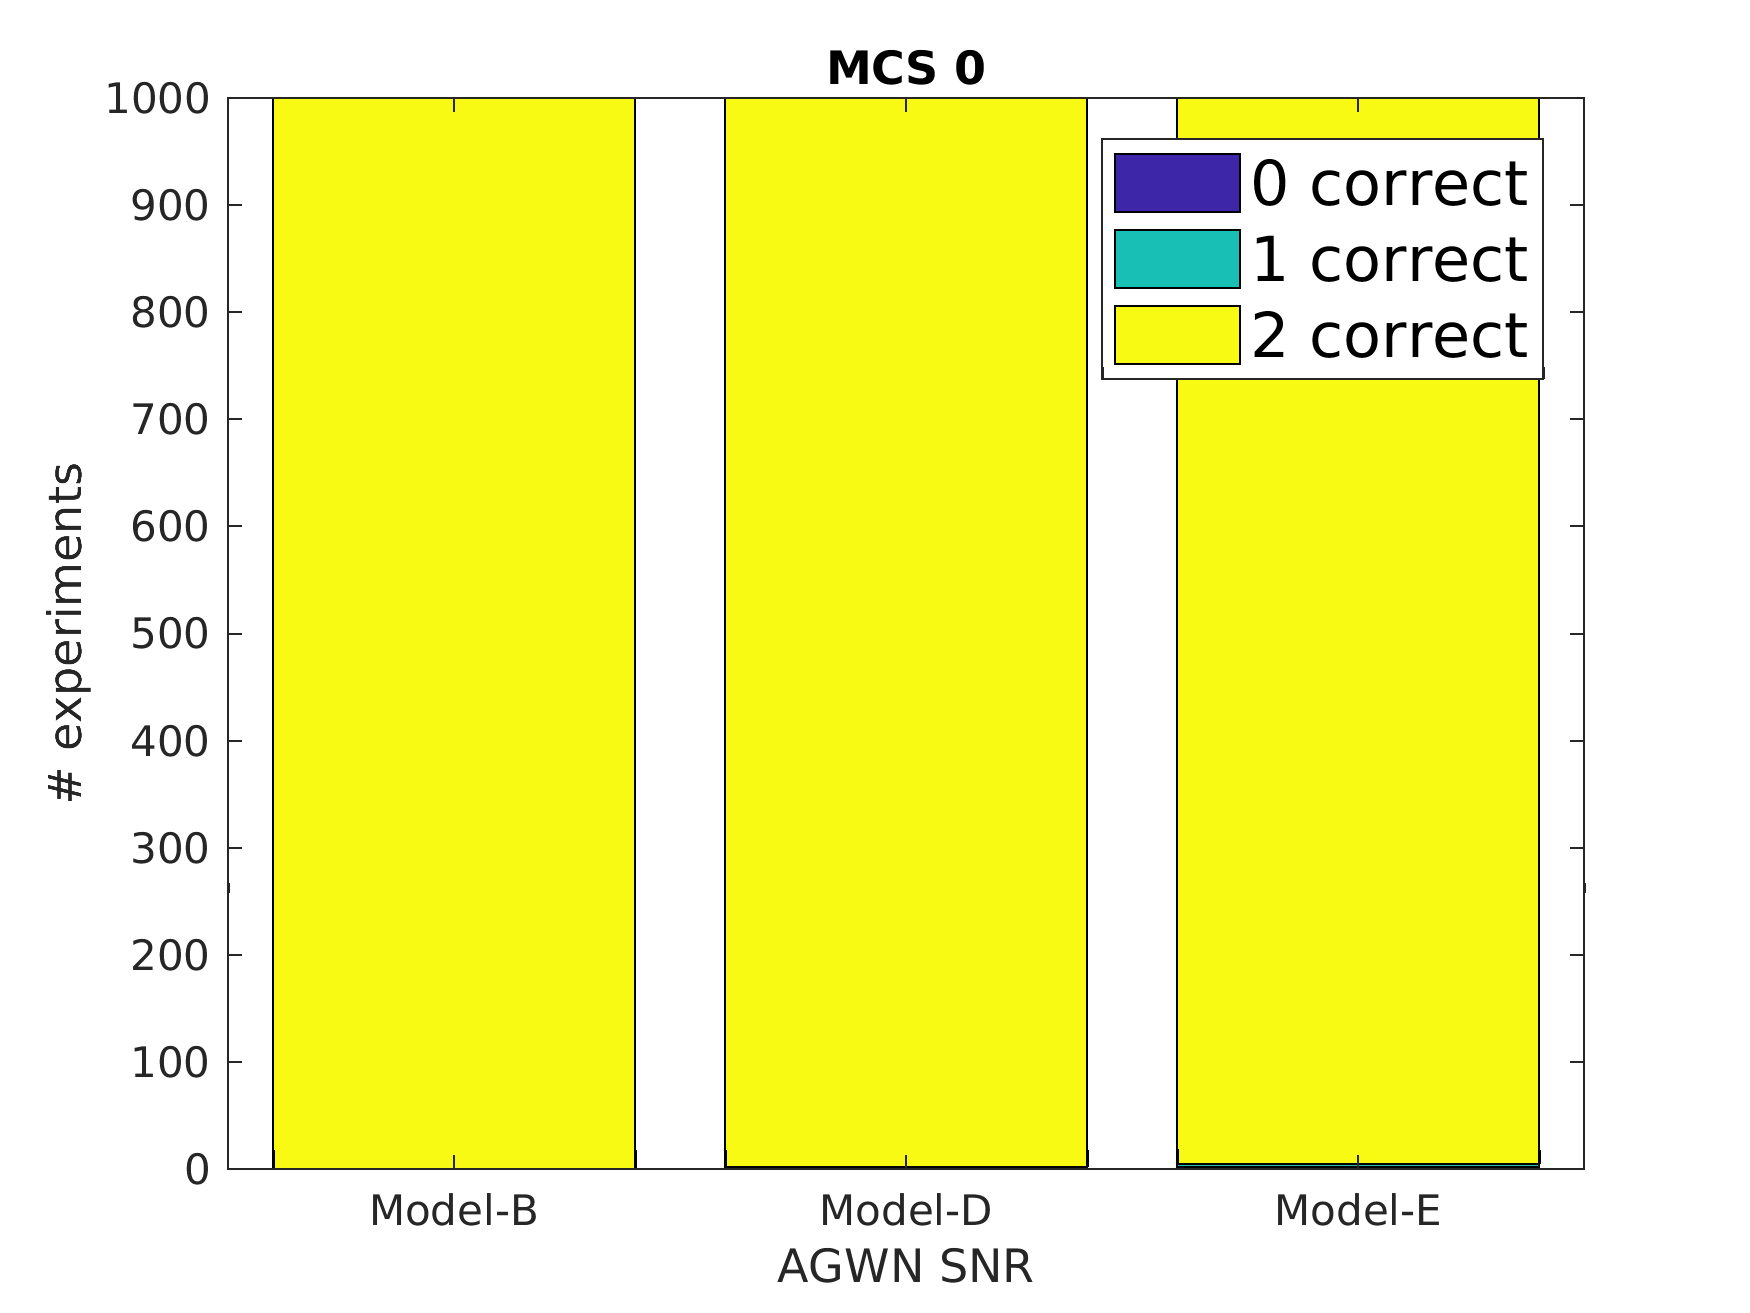
\includegraphics[height=0.52\textheight]{../../gfx/plots/tgn-mcs0} &
		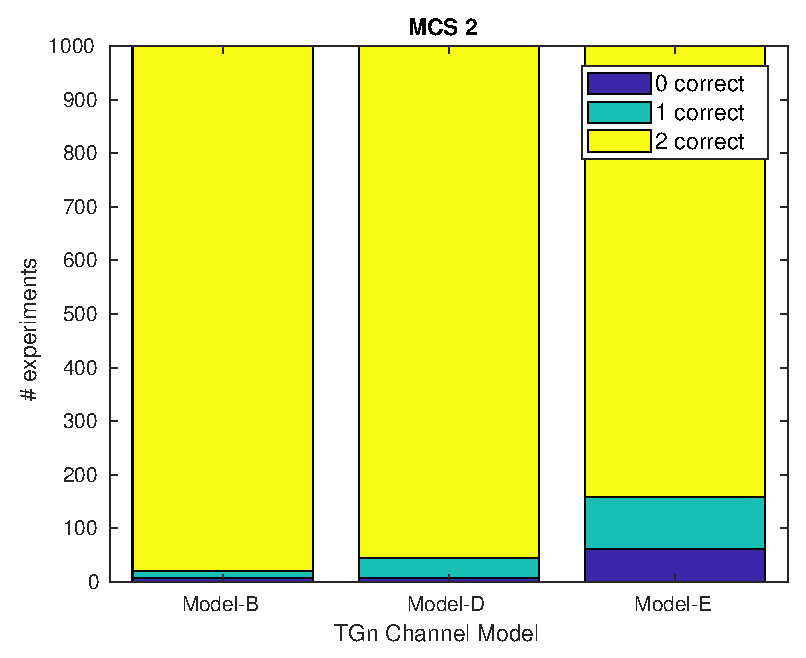
\includegraphics[height=0.52\textheight]{../../gfx/plots/tgn-mcs2} \\
		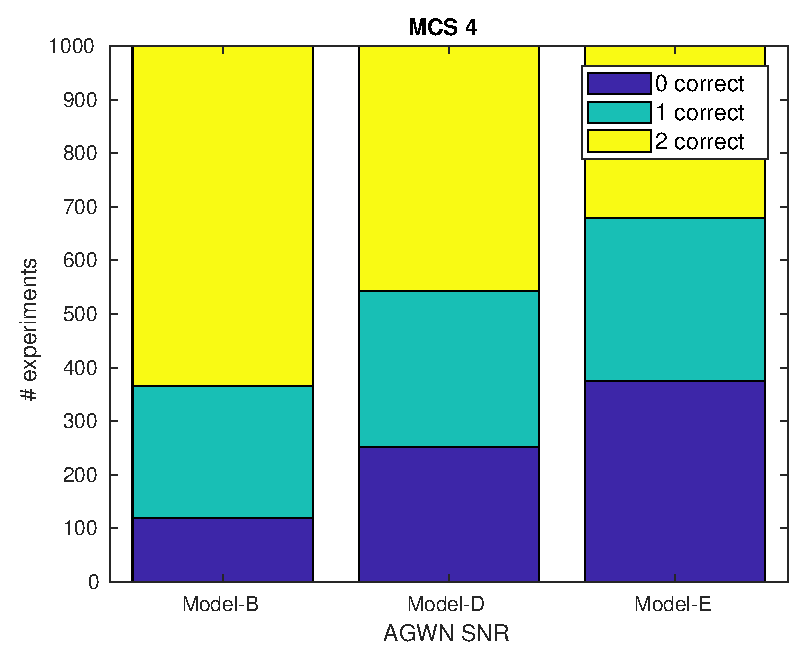
\includegraphics[height=0.52\textheight]{../../gfx/plots/tgn-mcs4} &
		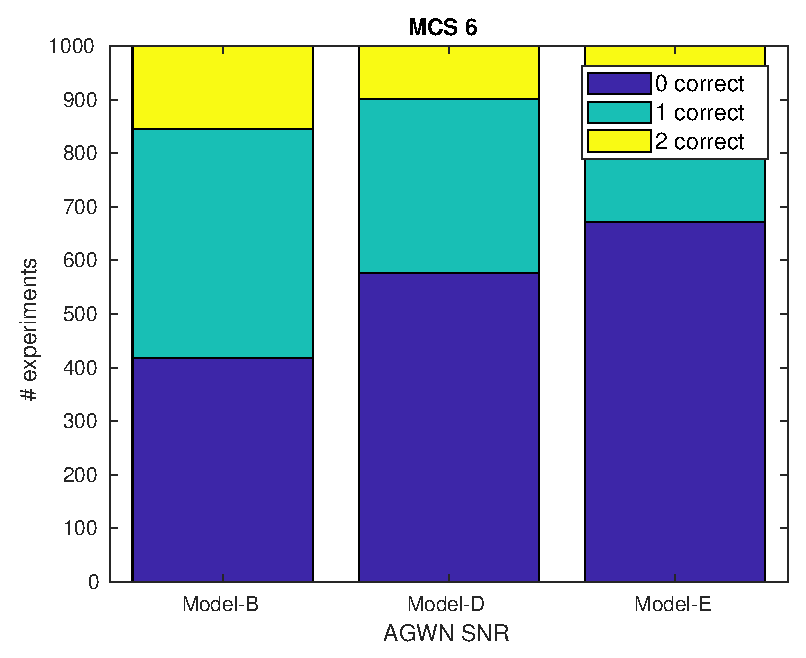
\includegraphics[height=0.52\textheight]{../../gfx/plots/tgn-mcs6} \\
	\end{tabular}
\end{figure}
\end{frame}


\begin{frame}
\frametitle{Results: Different MCSs on WARP Boards}
\begin{centering}
	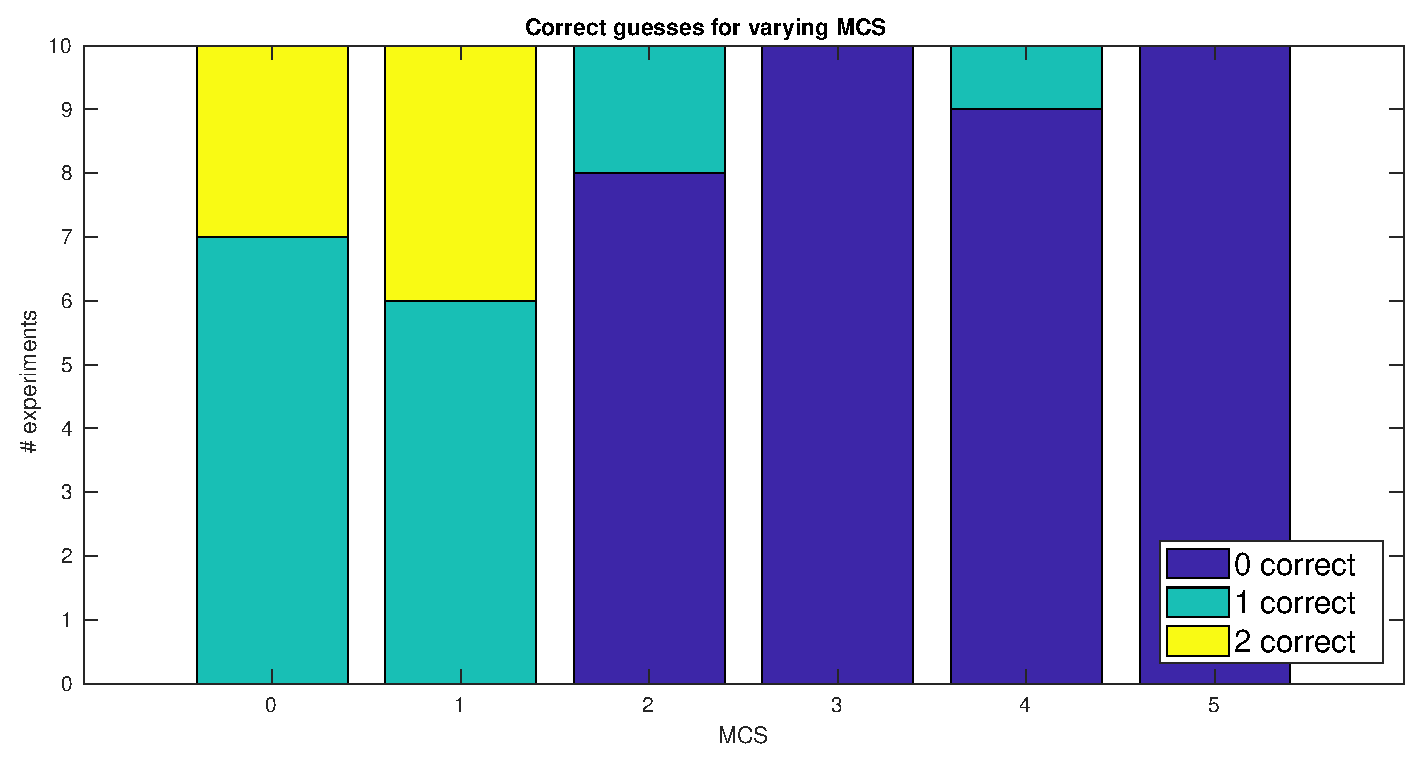
\includegraphics[width=11cm]{../../gfx/plots/warp-mcs}\\
\end{centering}
\end{frame}


\begin{frame}
\frametitle{Live Demo}
\begin{center}
	\vspace{1.45cm}
	\Huge U siriouz m8? Live demo no work!
\end{center}
\end{frame}


\begin{frame}
\frametitle{Discussion \& Conclusion}
\begin{itemize}
	\setlength\itemsep{1em}
	\item Important factors: MCS and Scrambler initialization
	\item Complexity: $ O(1016n) = O(n) $
	\item Real-time application possible
	\item Detection quality
	\begin{itemize}
		\setlength\itemsep{1em}
		\vspace{1em}
		\item Simulations: very good
		\item Hardware: only for MCSs 0 \& 1
	\end{itemize}
\end{itemize}
\end{frame}

	
\begin{frame}
\frametitle{Future Work}
\begin{itemize}
	\setlength\itemsep{1em}
	\item Quantitative noise evaluation with SDRs
	\item IEEE 802.11 n/ac/ax
	\item Implementation on mobile operating systems
	\item Generalization to more senders
\end{itemize}
\end{frame}


\begin{frame}
\frametitle{Thank you for your attention!}
\begin{center}
	\huge Questions and discussion\\
	\vspace{0,6cm}
	
\includegraphics[height=4cm]{assets/faq}
\end{center}
\end{frame}


\begin{frame}[allowframebreaks]
\frametitle{References}
\bibliographystyle{plain}
\bibliography{../../config/bibliography}
\end{frame}

\end{document}
